%% chapter01_introduction_slides.tex
%% Beamer slides for Chapter 1: Introduction
%% An Introduction to Universal Artificial Intelligence (2024)
%% Hutter, Quarel, Catt -- Taylor & Francis / CRC Press
%% Reader-friendly style: complete sentences, symbol explanations, worked examples
%% Compiled with: pdflatex -interaction=nonstopmode chapter01_introduction_slides.tex  (twice)
\documentclass[aspectratio=169,10pt]{beamer}

\usetheme{Madrid}
\usecolortheme{seahorse}

%% ── Packages ──────────────────────────────────────────────────────────────
\usepackage{amsmath,amssymb,amsfonts}
\usepackage{mathtools}
\usepackage{graphicx}
\usepackage{booktabs}
\usepackage{xcolor}
\usepackage{listings}
\usepackage{tikz}
\usetikzlibrary{arrows.meta,positioning,shapes.geometric,fit,backgrounds}

\graphicspath{{figures/}}

%% ── Python listing style ─────────────────────────────────────────────────
\lstdefinestyle{pycode}{
  language=Python,
  basicstyle=\ttfamily\scriptsize,
  numbers=left,
  numberstyle=\tiny\color{gray},
  frame=single,
  backgroundcolor=\color{gray!7},
  keywordstyle=\color{blue!70!black}\bfseries,
  commentstyle=\color{green!50!black}\itshape,
  stringstyle=\color{orange!80!black},
  showstringspaces=false,
  breaklines=true,
  tabsize=4,
  xleftmargin=1.5em,
  framexleftmargin=1.5em,
  aboveskip=4pt,
  belowskip=4pt,
}

%% ── Metadata ─────────────────────────────────────────────────────────────
\title[Ch.\,1 Introduction]{%
  \textbf{Chapter 1: Introduction}\\
  \normalsize An Introduction to Universal Artificial Intelligence}
\subtitle{Overview of the Book's Six Parts}
\author{Marcus Hutter, Elliot Catt, David Quarel}
\institute{Taylor \& Francis / CRC Press, 2024}
\date{}

\setbeamertemplate{footline}[frame number]
\setbeamertemplate{navigation symbols}{}

%% Helpful macros
\newcommand{\R}{\mathbb{R}}
\newcommand{\N}{\mathbb{N}}
\newcommand{\B}{\mathbb{B}}
\newcommand{\Pb}{\mathbb{P}}
\newcommand{\E}{\mathbb{E}}

%% ══════════════════════════════════════════════════════════════════════════
\begin{document}

%% ── Title frame ──────────────────────────────────────────────────────────
\begin{frame}
  \titlepage
\end{frame}

%% ── Outline ──────────────────────────────────────────────────────────────
\begin{frame}{Chapter Overview}
  \tableofcontents
\end{frame}

\AtBeginSection[]{\begin{frame}{Outline}\tableofcontents[currentsection]\end{frame}}

%% ══════════════════════════════════════════════════════════════════════════
\section{Why Build a Theory of Intelligence?}

\begin{frame}[allowframebreaks]{Inspiration from Nature and Human Civilization}
  \textbf{Learning by copying, then learning the rules.} Humans have always
  learned from nature: the airplane was inspired by birds, the camera mimics
  the eye (the aperture moderates light the way a pupil does, and the
  photosensitive sensor mimics the retina), and hook-and-loop fasteners copy
  the hooked barbs of a thistle bush. Over time we stopped merely copying
  nature's designs and started learning the \emph{rules} by which nature
  works, so that we could improve on them: we domesticate wolves into dogs,
  selectively breed crops for higher yield, and directly edit genetic code.

  \vspace{0.3cm}
  \textbf{The pattern behind civilization.} Humanity first recognized
  patterns (crop rotation improves yield) long before understanding why they
  worked. Later we built theories and laws that explain observations and let
  us predict new ones. This created a positive feedback loop: more knowledge
  lets us extend our capabilities further, which in turn lets us gain more
  knowledge. Agriculture freed people to specialize; writing let ideas travel
  across time; calculus, once known to only a handful of experts, is now
  routine high-school material.

  \framebreak

  \textbf{The human brain and mind.} All of these innovations share a common
  source: human intelligence, meaning the ability to reason, strategize, and
  plan ahead so as to steer the world toward states we prefer. We would like
  to do to the brain what the combine harvester did to the ox: build an
  artificial version that can think and plan for us. Intelligence remains one
  of the least understood natural phenomena --- neuroscience can localize
  which brain regions are active for vision, speech, or memory, but this
  provides, at best, coarse answers about how thought and consciousness
  actually arise.

  \vspace{0.3cm}
  \textbf{Why theory, not just engineering.} Sophisticated inventions
  typically require theory before reliable engineering is possible. A digging
  stick needs no theory of mechanics to build; but nobody built a rocket or a
  computer by connecting parts haphazardly until something worked. The Turing
  machine predates practical computers by a decade, and the theory of space
  flight was mature well before the first successful rocket launch. Right
  now, artificial general super-intelligence (a term explained on the next
  slide) is still very much at the theory stage --- which is exactly the gap
  this book tries to fill.
\end{frame}

\begin{frame}{Proliferation of AI Terminology}
  \small
  As AI capabilities have grown, the community has needed increasingly
  precise terms to describe \emph{how broad} and \emph{how strong} a
  system's intelligence is.

  \begin{block}{Five Levels of Machine Intelligence}
    \begin{itemize}\itemsep1pt
      \item \textbf{ANI} (Artificial Narrow Intelligence): performs well in a
        single narrow domain (board games, transcription, image
        recognition).
      \item \textbf{Proto-AGI}: a system --- such as today's Large Language
        Models (LLMs) --- generalizing across many problems, without being
        fully general.
      \item \textbf{AGI} (Artificial General Intelligence): performs
        virtually all intellectual tasks as well as a typical human.
      \item \textbf{ASI} (Artificial Super-Intelligence): exceeds most
        humans in a reasonably broad domain (e.g., composing like Mozart,
        deriving mathematics to rival Gauss).
      \item \textbf{AGSI} (Artificial General Super-Intelligence): AGI $+$
        ASI --- ``greatly exceeds the cognitive performance of humans in
        virtually all domains of interest'' (Bostrom).
    \end{itemize}
  \end{block}
  Plain English: each level up the list means the system is good at more
  \emph{kinds} of tasks (breadth) and/or is better \emph{than humans} at them
  (depth). \textbf{Universal Artificial Intelligence (UAI)} is the formal
  theory this book builds, and \textbf{AIXI} is a mathematically
  well-defined AGSI agent that the theory constructs and proves properties
  about.
\end{frame}

\begin{frame}{AI Capability Levels: The Table}
  \begin{table}
    \centering
    \begin{tabular}{lccc}
      \toprule
      \textbf{AI-Type} & \textbf{\#domains} & \textbf{Intelligence Level} & \textbf{Achieved} \\
      \midrule
      ANI        & one         & idiot savant & 1980--1997 \\
      Proto-AGI  & many        & human        & 2023--2028 \\
      AGI        & most        & smart        & 2028--2038 \\
      ASI        & some/many   & genius       & 2038--2042 \\
      AGSI       & nearly all  & humanity     & 2042--2048 \\
      \midrule
      UAI/AIXI   & all         & maximal      & 2000/theory \\
      \bottomrule
    \end{tabular}
  \end{table}
  Plain English: reading down the table, each row needs to succeed in more
  domains (\#domains) at a higher intelligence level than the last. The
  final row, \textbf{UAI/AIXI}, is the book's theoretical reference point:
  a formal notion of ``maximal'' intelligence across \emph{all} domains,
  that has existed as a theory since the year 2000, even though no
  practical algorithm achieves it.
\end{frame}

\begin{frame}{AI Capability Levels: A Timeline}
  \small
  \begin{center}
    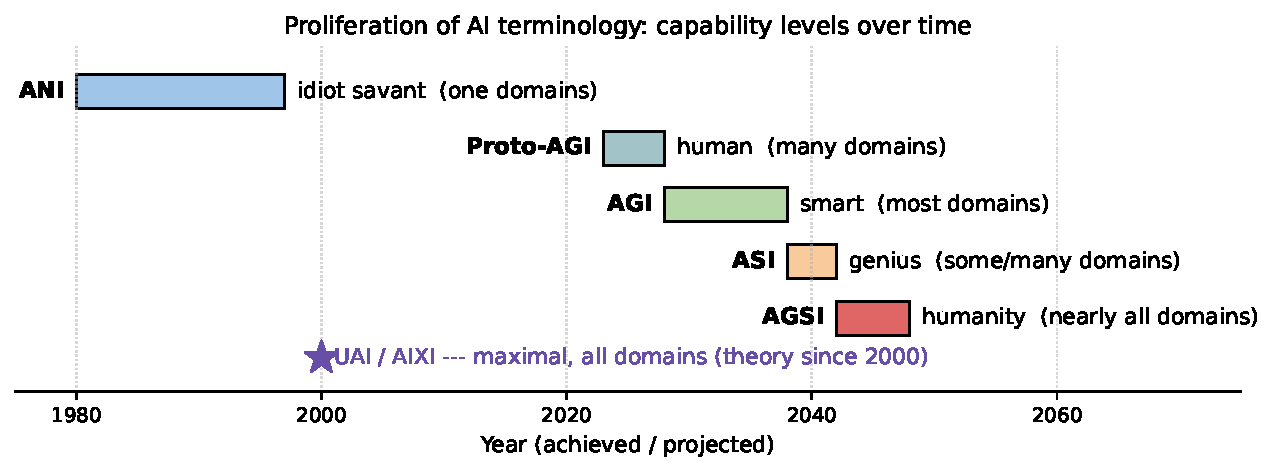
\includegraphics[width=0.8\textwidth]{ai_timeline}
  \end{center}
  Plain English: the bars are the book's own (necessarily speculative)
  estimate of \emph{when} each capability level might be reached in
  practice. The star marks that \textbf{UAI/AIXI already exists today ---
  but only as a theory}, not as a practical algorithm; it acts as the
  ``maximal'' reference point that every other level is measured against.
\end{frame}

\begin{frame}[allowframebreaks]{Artificial Intelligence and Why Theory Matters}
  \textbf{Sophisticated inventions require theory.} While it is hard to
  predict the internal structure of a future AGSI, this book is primarily
  concerned with a theory of the \emph{behavior} of such agents, which can
  guide practical realizations. Many innovations are simple enough to build
  without deep theory (a digging stick), but the more complex a device
  becomes, the more fragile it is to mistakes: an almost-complete shovel can
  still dig; an almost-complete computer is an expensive paperweight, and an
  almost-complete rocket explodes on the launch pad.

  \vspace{0.3cm}
  \textbf{A mathematical theory of (super)intelligence.} It may seem
  implausible that a single theory could capture reasoning, creativity,
  curiosity, pattern recognition, problem solving, memorization, planning,
  and learning all at once. Yet this book will show that Universal
  Artificial Intelligence encapsulates any reasonable definition of
  intelligence, and that within this theory there exists an agent that can
  be shown to be, in a precise sense, ``maximally intelligent'': this agent
  is called \textbf{AIXI}.

  \framebreak

  \textbf{The structure of the book.} The remainder of this introduction
  previews the six parts of the book, each building on the last: background
  mathematics, algorithmic prediction, a family of universal agents, ways
  to approximate those (incomputable) agents, alternative non-Bayesian
  approaches, and finally safety and philosophical discussion.

  \begin{center}
    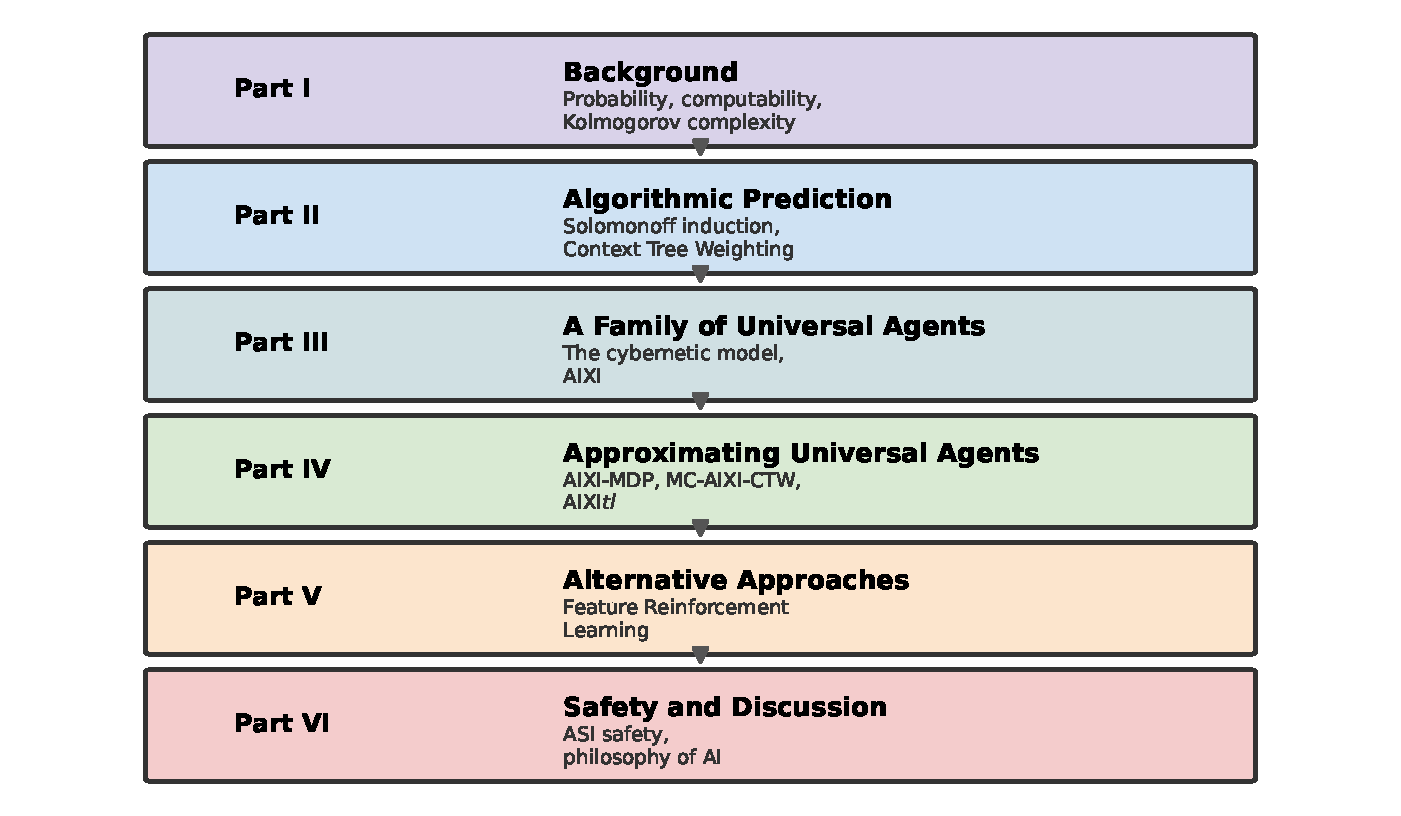
\includegraphics[width=0.48\textwidth]{book_structure}
  \end{center}
\end{frame}

%% ══════════════════════════════════════════════════════════════════════════
\section{Part I --- Background}

\begin{frame}[allowframebreaks]{Part I: Background}
  Universal Artificial Intelligence builds on results from many established
  theories: Bayesian probability, computability theory, complexity theory,
  algorithmic information theory, sequential decision theory, reinforcement
  learning, and game theory. Chapter 2 of the book gives an extensive
  background chapter; here is a preview of \emph{why} each ingredient is
  needed.

  \begin{block}{Binary Strings}
    Deep down, computers operate exclusively on bits (binary digits) and bit
    sequences. UAI theory assumes all data has been preprocessed into binary
    strings. \emph{Prefix-free codes} let concatenated, transmitted strings
    be uniquely decoded again. Since all real-world sequences are finite, but
    asymptotic convergence proofs need a notion of an unboundedly long
    sequence, the theory also considers \emph{infinite} binary sequences.
  \end{block}

  \framebreak

  \begin{block}{Measure Theory and Probability Theory}
    The world an agent experiences is not deterministic --- it contains
    (quantum-physical) random processes. Probability theory models this
    uncertainty mathematically. Simple combinatorial ``high-school''
    probability is not sufficient for the sophisticated arguments in this
    book; rigorous probability theory is built on \emph{measure theory},
    which the book uses sparingly and tries to keep to a minimum.
  \end{block}

  \begin{block}{Statistical Inference and Estimation, Bayesian Probability}
    Agents only have partial knowledge of the world and must infer the
    unknown probability distribution that generated their observations. For
    simple independent and identically distributed (i.i.d.) data, frequency
    estimates work well; for harder problems, maximum likelihood estimation
    is a good default --- but it breaks down in the most difficult
    situations. \emph{Bayesian probability theory} models the agent's own
    uncertainty as a probability distribution (a \emph{belief}) over
    possible world-models, and updates that belief with new evidence via
    \textbf{Bayes' Law}, a completely general and optimal learning rule.
  \end{block}

  \framebreak

  \begin{block}{Information Theory, Coding, and Computability Theory}
    Classical Shannon information theory uses \emph{entropy} to measure the
    expected code length needed to compress data from a random source.
    \emph{Computability theory} formalizes the concept of an algorithm via
    universal Turing machines, which can emulate any computable process ---
    the theoretical reason a single smartphone can run any program we like.
  \end{block}

  \begin{block}{Kolmogorov Complexity}
    \textbf{Occam's razor} says we should prefer simpler explanations.
    Kolmogorov complexity makes this precise: it measures the complexity of
    a binary sequence (or, more generally, of any object) by the length of
    the shortest program that produces it. This gives a fully general,
    optimal notion of ``simplicity'' that does not depend on the choice of
    description language beyond an additive constant. Plugged into a
    Bayesian sequence predictor, this becomes the \textbf{Solomonoff
    predictor}; combined with sequential decision theory (Chapter 6), it
    leads to the agent \textbf{AIXI}.
  \end{block}

  \begin{block}{Miscellaneous}
    The background chapter also covers various \emph{distance measures}
    between probability distributions (absolute distance, 2-norm,
    Kullback--Leibler divergence, Hellinger distance), \emph{semimeasures}
    (a workaround for programs that may never halt), and how to handle
    probability-zero events, which appear throughout the book. This
    concludes the background preview --- Chapter 2 covers all of it in
    full mathematical detail.
  \end{block}
\end{frame}

\begin{frame}[fragile]{Python: Bayes' Law in Action}
  A small numeric illustration of Bayesian updating --- the mechanism behind
  Part I's ``Bayesian probability theory'' --- using two candidate coins.

  \begin{lstlisting}[style=pycode]
# Two hypotheses about a coin: fair (p=0.5) vs biased (p=0.8 heads)
# Prior belief: we think "fair" is a bit more likely a priori.
prior = {"fair": 0.6, "biased": 0.4}
p_heads = {"fair": 0.5, "biased": 0.8}

def bayes_update(prior, p_heads, observation):
    # likelihood of the observation ("H" or "T") under each hypothesis
    like = {h: (p_heads[h] if observation == "H" else 1 - p_heads[h])
            for h in prior}
    unnorm = {h: prior[h] * like[h] for h in prior}
    z = sum(unnorm.values())              # normalizing constant
    return {h: unnorm[h] / z for h in prior}

belief = prior
for toss in ["H", "H", "H", "H"]:          # four heads in a row
    belief = bayes_update(belief, p_heads, toss)
    print(f"after {toss}: fair={belief['fair']:.3f}  biased={belief['biased']:.3f}")
  \end{lstlisting}
  Output after four heads: belief shifts from 60\%/40\% (fair/biased) toward
  roughly 24\%/76\% --- each additional head makes the ``biased'' hypothesis
  relatively more likely, exactly as Bayes' Law prescribes.
\end{frame}

%% ══════════════════════════════════════════════════════════════════════════
\section{Part II --- Algorithmic Prediction}

\begin{frame}{Part II: What Is Prediction?}
  \textbf{Prediction} is the ability to accurately estimate the outcome of
  future events based on past ones. We formalize this as predicting the next
  element (or elements) of a sequence.

  \begin{block}{A Motivating Puzzle}
    Given the sequence
    \[
      3,\ 1,\ 4,\ 1,\ 5,\ 9
    \]
    what is the next element? An observant reader may notice these are the
    first six digits of $\pi$ (pi) in base 10, suggesting the next digit is
    2. But this is not the only continuation consistent with the data: the
    decimal expansion of $355/113$ (a famous rational approximation of $\pi$)
    also starts $3,1,4,1,5,9$, and is arguably just as simple.
  \end{block}
  Plain English: prediction is necessary for intelligence but not
  sufficient, because it is measured as a function of \emph{actions}, whereas
  pure prediction assumes the predictions themselves do not change the
  environment.
\end{frame}

\begin{frame}{Occam's Razor and Epicurus' Principle}
  \begin{block}{Epicurus' Principle of Multiple Explanations}
    \emph{Keep all theories consistent with the observations.}
  \end{block}
  We must not discard the possibility that $355/113$ (or something else
  entirely) is the true continuation --- but this does not mean all
  consistent continuations are equally likely.

  \begin{block}{Occam's Razor}
    \emph{Entities should not be multiplied beyond necessity}, which we
    interpret here as: \emph{Keep the simplest theory consistent with the
    observations.}
  \end{block}
  Plain English: any number could in principle be next, but we bias our
  prediction toward the outcomes produced by \emph{simpler} explanations. As
  we observe more digits, hypotheses inconsistent with the new data get ruled
  out --- a process the book calls \textbf{learning by elimination}. More
  digits of the true sequence will soon distinguish $\pi$ from $355/113$.
\end{frame}

\begin{frame}{Bayesian Sequence Prediction and Solomonoff Induction}
  \small
  \begin{block}{The Mechanism: Bayes' Law with an Occam Prior}
    Given a prior belief $P(O{=}o)$ over sequences $o$ in some reference
    class, the posterior belief among sequences not yet ruled out by the
    data is a rescaled version of the prior (probabilities again sum to
    1). If sequences may be noisy, each gets a \emph{likelihood}, which
    multiplies the prior to give the posterior --- this multiplicative
    rule is \textbf{Bayes' Law}.
  \end{block}
  The only remaining choice is the prior itself. Motivated by Occam's razor,
  we bias the prior toward ``simpler'' outcomes, formalized via Kolmogorov
  complexity. This combination is \textbf{Solomonoff Induction}, a formal
  theory of inductive inference based on \emph{algorithmic probability}.

  \begin{center}
    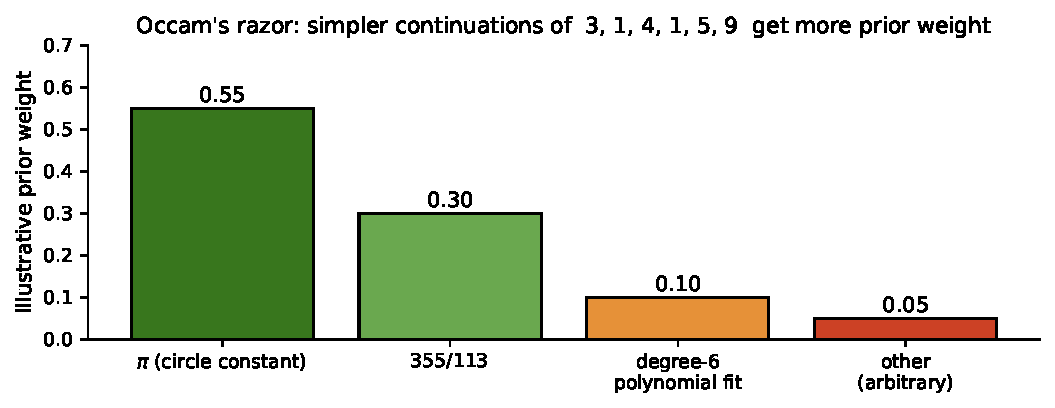
\includegraphics[width=0.5\textwidth]{occam_weights}
  \end{center}
  \footnotesize Plain English (figure): simpler continuations of
  $3,1,4,1,5,9$ (like ``it's $\pi$'') receive more prior weight, but no
  consistent continuation ever gets zero weight.
\end{frame}

\begin{frame}{Why Occam's Razor Works: The Orbit of Mars}
  \begin{block}{A Historical Illustration}
    In the mid-19th century, Urbain Le Verrier noticed that the orbit of
    Mars \emph{precesses} (its major axis slowly rotates) in a way classical
    mechanics could not explain. One could ``patch'' classical mechanics
    with an extra rule just for this edge case, but doing so dramatically
    increases the theory's complexity. Einstein's general relativity instead
    explained the precession (and other phenomena, like light deflection
    near massive objects) from \emph{fewer} core assumptions, with classical
    mechanics emerging as a special case.
  \end{block}
  Plain English: a theory patched with extra special cases to fit
  observations is more complex and, by Occam's razor, less likely to be
  correct than a theory that explains the same observations from simpler
  first principles. Solomonoff turned this intuition into a mathematically
  precise procedure: a prior over a countably infinite model class must
  assign more probability to some outcomes than others, and choosing that
  prior according to simplicity means prediction errors are proportional to
  the complexity of the (unknown) true environment. In a strong sense,
  Solomonoff induction is the \emph{best possible} predictor for unknown
  stochastic sources --- an ideal gold standard that practical predictors
  strive toward.
\end{frame}

\begin{frame}{Context Tree Weighting and Its Extensions}
  \begin{block}{Context Tree Weighting (CTW)}
    CTW is a practical Bayesian predictor whose reference class is the set
    of all \emph{variable-order Markov models} --- models where the
    probability of the next symbol depends only on a bounded number of the
    most recent symbols. CTW uses a \emph{tree structure} to efficiently
    update its belief over this whole model class as symbols are observed.
    Each hypothesis (each tree) is weighted by a prior related to the length
    of a binary encoding of that tree --- the same Occam-style bias as
    Solomonoff induction, but restricted to a computationally tractable
    model class.
  \end{block}
  Extensions mentioned in the book include \textbf{Context Tree Switching}
  (switches between different distributions depending on context),
  \textbf{Partition Tree Weighting} (piecewise-stationary sources, useful
  e.g. for compressing mixed-file-type archives), the \textbf{Forget-me-not
  Process} (remembers statistics of past pieces), and \textbf{Context Tree
  Maximization} (extracts the single most plausible model when mixing many
  models is undesirable).
\end{frame}

\begin{frame}[fragile]{Python: A Toy Solomonoff-Style Predictor}
  A tiny numeric demonstration of Occam-weighted prediction: three
  candidate ``programs'' (rules) explain the data so far, each weighted by
  $2^{-\ell}$ where $\ell$ is its description length (in bits) --- shorter
  programs get exponentially more prior weight, then all get renormalized
  by Bayes' Law after checking which remain consistent with new data.

  \begin{lstlisting}[style=pycode]
data_so_far = [3, 1, 4, 1, 5, 9]

# Each "program" is (description_length_in_bits, rule_function)
programs = [
    (4,  lambda seq: [3,1,4,1,5,9,2,6,5][len(seq)]),      # "digits of pi"
    (6,  lambda seq: [3,1,4,1,5,9,2,9,2][len(seq)]),      # "digits of 355/113"
    (10, lambda seq: seq[-1]),                            # "repeat last digit"
]

def prior_weight(length_bits):
    return 2 ** (-length_bits)                # Occam prior: shorter = more likely

weights = {i: prior_weight(L) for i, (L, _) in enumerate(programs)}
total = sum(weights.values())
posterior = {i: w / total for i, w in weights.items()}    # normalize to sum to 1

for i, (L, rule) in enumerate(programs):
    print(f"program {i} (length {L} bits): prior weight "
          f"{posterior[i]:.3f}, predicts next digit = {rule(data_so_far)}")
  \end{lstlisting}
  The 4-bit ``digits of $\pi$'' program dominates the mixture (about 70\% of
  the total weight here) purely because it is shortest --- illustrating how
  an Occam prior concentrates belief on simple, so-far-consistent rules.
\end{frame}

%% ══════════════════════════════════════════════════════════════════════════
\section{Part III --- A Family of Universal Agents}

\begin{frame}{Part III: From Prediction to Action}
  Intelligence is more than predicting well; it also requires \emph{acting}
  well. ``Acting well'' can mean many things: achieving a predetermined
  goal, maintaining an objective, minimizing a loss function, respecting
  constraints, acting rationally, or making correct decisions given
  available information. The book captures all of these within a single
  framework: the \textbf{cybernetic model}.
\end{frame}

\begin{frame}{The Cybernetic Model}
  \begin{block}{Agent--Environment Interaction}
    An \emph{agent} $\pi$ (pi, denoting the agent's \emph{policy}) interacts
    with an \emph{environment} $\mu$ (mu) over cycles $t=1,2,\ldots,m$. In
    cycle $t$, the agent takes action $a_t$ based on the past percepts
    $e_1 \ldots e_{t-1}$, where the percept $e_k := o_k r_k$ bundles together
    an observation $o_k$ and a real-valued reward $r_k$. The environment then
    provides a fresh observation $o_t$ and reward $r_t$, and cycle $t+1$
    begins.
  \end{block}
  \begin{center}
    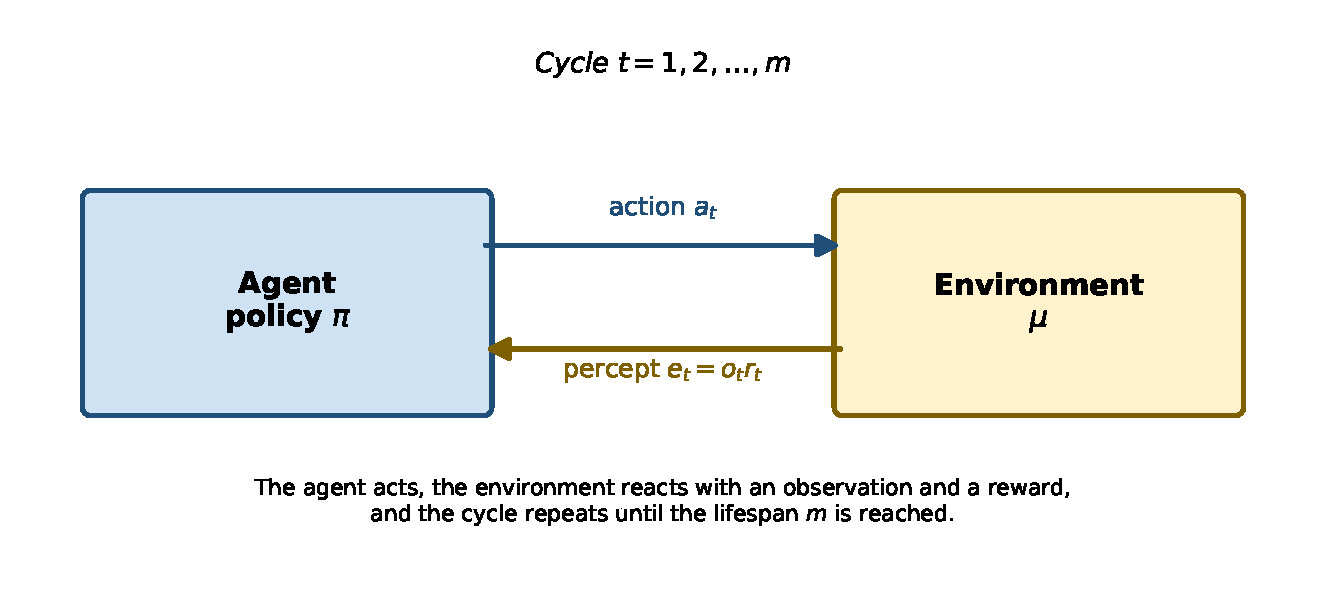
\includegraphics[width=0.75\textwidth]{cybernetic_loop}
  \end{center}
  Plain English: the agent and environment take turns. The agent's policy
  $\pi$ may use the \emph{entire} past history (not just the most recent
  observation), which is why this is called \textbf{history-based} or
  \textbf{general reinforcement learning}, in contrast to most reinforcement
  learning, which assumes Markov environments (future depends only on the
  most recent observation and action).
\end{frame}

\begin{frame}{The Goal of the Agent: Value}
  The goal of the agent is to maximize its \emph{expected total reward},
  called \textbf{value}. This single mechanism can encode many different
  goals just by choosing the reward and environment appropriately: to make
  an agent play chess well, issue $+1$ for winning and $-1$ for losing, and
  0 otherwise. Human intelligence itself is arguably a by-product of an
  evolutionary arms race optimizing for reproductive fitness, with pleasure
  and pain acting as ``reward signals'' for behaviors correlated with
  survival and reproduction.

  \begin{block}{Known vs.\ Unknown Environment}
    If the agent already knows which environment $\mu$ it is interacting
    with, it can (in principle) deduce the best action --- e.g., chess can be
    solved by the \emph{minimax} algorithm given perfect play, even though
    this is computationally intractable in practice. The interesting case for
    AG(S)I is when the agent does \emph{not} know the environment and must
    learn it from experience, the way a person learns the rules of a new
    video game purely by playing it.
  \end{block}
\end{frame}

\begin{frame}{AIXI: The Universal Bayes-Optimal Agent}
  We assume only that the true environment is \emph{computable}, and take
  the reference class of \emph{all} computable environments --- guaranteeing
  the true environment is included. Combining Solomonoff induction (for
  prediction) with optimal sequential decision-making gives \textbf{AIXI}.

  \begin{block}{The AIXI Equation}
    \[
      a_t \;:=\; \operatorname*{argmax}_{a_t}\sum_{o_t r_t}\ \cdots
      \operatorname*{max}_{a_m}\sum_{o_m r_m}\ [r_t + \ldots + r_m]
      \sum_{p:\, U(p,a_1\ldots a_m)\to o_1 r_1 \ldots o_m r_m} 2^{-\mathrm{length}(p)}
    \]
    where $t{=}$now, $a{=}$action, $o{=}$observation, $r{=}$reward,
    $U{=}$universal Turing machine, $p{=}$program, $m{=}$lifespan.
  \end{block}
  Plain English: AIXI picks the action $a_t$ that maximizes its total
  \emph{expected} future reward $r_t + \ldots + r_m$. For each hypothetical
  future, a program $p$ that reproduces the percepts seen so far contributes
  to the average with weight $2^{-\mathrm{length}(p)}$ --- shorter (simpler)
  explanations count more, exactly as in Solomonoff induction. The
  alternating $\max$ and $\sum$ operators interleave ``choose the best
  action'' with ``average over what the environment might do'', evaluated
  in chronological order (similar to minimax in games).
\end{frame}

\begin{frame}{Understanding AIXI: Why It Matters}
  One can fix any finite action/perception space, any reasonable universal
  Turing machine $U$, and any (large) finite lifespan $m$ --- this completely
  and uniquely defines AIXI's actions $a_t$. AIXI is \textbf{limit-computable}
  (all quantities in the formula are, in principle, knowable, even though
  Solomonoff induction itself is incomputable in general).

  \begin{block}{The Book's Central Claims About AIXI}
    \begin{itemize}
      \item AIXI eventually acts as well as the optimal \emph{informed} agent
        that already knows the true environment in advance.
      \item Since Bayes' Law is a maximally data-efficient learning rule, and
        AIXI is a universal Bayesian learner, AIXI learns as fast as
        theoretically possible.
      \item AIXI is incomputable (since Solomonoff induction is), but serves
        as a \emph{gold standard} for building practical approximations ---
        much like exhaustive minimax for chess paved the way for practical
        chess engines.
    \end{itemize}
  \end{block}
  The name \textbf{AIXI} is pronounced [aiksi] or ['aiksi:], and can be read
  as: AI based on Solomonoff's distribution $\xi$ (Greek letter Xi); or AI
  (I)nduction crossed with (X) action.
\end{frame}

\begin{frame}{Variations of AIXI and the Multi-Agent Setting}
  Bayes-optimality is a sensible but not the \emph{only} optimality criterion
  for intelligent agents.

  \begin{block}{Selected Variations}
    \begin{itemize}
      \item \textbf{Knowledge Seeking Agent (KSA)}: replaces reward-seeking
        with maximizing expected future \emph{information gain} --- it takes
        actions leading to the most ``surprising'' observations.
      \item \textbf{Optimism/pessimism}: acting \emph{optimistically}
        (assuming the best realistically possible environment) can achieve
        optimal behavior, unlike in pure prediction.
      \item \textbf{Thompson sampling}: acts optimally with respect to a
        single environment \emph{sampled} from the posterior belief, rather
        than a full Bayesian mixture.
      \item \textbf{BayesExp}, \textbf{Inq}, \textbf{SelfAIXI},
        \textbf{AIXItl}: intersperse Bayes-optimal actions with extra
        exploration, or predict their own future actions.
    \end{itemize}
  \end{block}
  \textbf{Multi-agent setting.} This book mostly treats a single agent in an
  environment, but since UAI makes almost no assumptions on environment
  structure, other agents (including humans) can simply be part of the
  environment. This connects to game theory (Nash equilibria) and raises the
  \emph{Grain of Truth} problem: Bayes-optimality requires the true
  environment to be in the considered model class, yet a Bayes-optimal agent
  is typically \emph{not} in its own model class. A superclass of AIXI based
  on \emph{reflective oracles} resolves this by being closed under Bayesian
  optimality.
\end{frame}

\begin{frame}[fragile]{Python: A Miniature AIXI-Style Agent}
  A brute-force illustration of the AIXI equation's mechanics on a tiny
  two-action, one-step problem with three candidate ``environment
  programs'' of different lengths (shorter = higher prior weight
  $2^{-\mathrm{length}(p)}$), each predicting a reward for each action.

  \begin{lstlisting}[style=pycode]
actions = ["left", "right"]

# programs: (bit-length, {action: predicted_reward})
programs = [
    (2, {"left": 1.0, "right": 0.0}),   # short & simple: "left is good"
    (3, {"left": 0.0, "right": 1.0}),   # short & simple: "right is good"
    (8, {"left": 0.9, "right": 0.9}),   # long & complex: "both are fine"
]
weights = [2 ** (-L) for L, _ in programs]
total_w = sum(weights)

def expected_reward(action):
    # weighted average of the reward each program predicts for this action
    return sum(w * probs[action] for w, (_, probs) in zip(weights, programs)) / total_w

best_action = max(actions, key=expected_reward)
for a in actions:
    print(f"action={a:5s}  expected reward = {expected_reward(a):.3f}")
print("AIXI-style choice: argmax action =", best_action)
  \end{lstlisting}
  Because the two short, mutually-contradicting programs dominate the
  mixture, the agent's decision is driven mostly by whichever short program
  favors an action --- the long ``safe'' program contributes little, exactly
  as the $2^{-\mathrm{length}(p)}$ weighting in the AIXI equation intends.
\end{frame}

%% ══════════════════════════════════════════════════════════════════════════
\section{Part IV --- Approximating Universal Agents}

\begin{frame}{Part IV: Why We Need Approximations}
  AIXI itself cannot be computed directly, but we can implement
  \emph{weaker} agents that approximate it. Unsurprisingly, the better the
  approximation, the harder it is to compute.

  \begin{block}{AIXI-MDP}
    Considers only \emph{Markov environments}, i.e., environments where the
    next observation and reward depend only on the previous observation and
    action (a \emph{Markov Decision Process}, MDP). AIXI-MDP is computable
    and performs well on Markov environments, but struggles on more complex
    ones, since it can only learn the closest Markov approximation to the
    true environment.
  \end{block}

  \begin{block}{Monte Carlo AIXI with Context Tree Weighting (MC-AIXI-CTW)}
    Uses CTW (Part II) to efficiently update beliefs over the class of all
    \emph{variable-order Markov environments}, combined with Monte-Carlo
    Tree Search for planning. This combination lets the agent learn and
    perform well on substantially more complex environments than AIXI-MDP.
  \end{block}
\end{frame}

\begin{frame}{Time- and Space-Bounded AIXI: AIXI$tl$}
  AIXI-MDP and MC-AIXI-CTW both fix a specific, immutable class of
  environments, even if more computation becomes available, and separately
  approximating (Solomonoff) learning and (expectimax) planning can itself
  be very suboptimal.

  \begin{block}{AIXI$tl$}
    The resource-constrained version of AIXI. It searches through program
    space and selects the policy of size at most $l$ that acts in time at
    most $t$ per interaction cycle, while performing as well as the best
    such $(l,t)$-bounded policy. AIXI$tl$ runs in time $O(2^l t)$ and is a
    \emph{compute-optimal anytime algorithm} that approaches AIXI as $t$ and
    $l \to \infty$.
  \end{block}
  Plain English: bigger $l$ and $t$ mean ``search over more, and more
  time-expensive, candidate policies,'' at exponentially increasing cost in
  $l$ but only linear cost in $t$. The hard remaining problem is that even
  \emph{evaluating} whether a candidate program is a good policy is itself
  incomputable in general --- solved by carefully designing a lower
  semicomputable universal value function, and requiring that policies
  provably conservatively evaluate themselves.
\end{frame}

\begin{frame}{(In)computability of AIXI}
  AIXI at least lies within the \textbf{arithmetic hierarchy}, a way of
  classifying how ``far'' from computable a quantity is by counting
  alternating quantifiers needed to define it.

  \begin{block}{How Incomputable Is AIXI?}
    Carelessly taking various limits (limit-computable environments,
    averaging over infinitely many of them, infinite horizon, incomputable
    discounting, \ldots) shows that all versions of AIXI are, at worst, at
    level $\Delta^0_4$ (Delta-zero-four) of the arithmetic hierarchy. With
    more care, some versions of AIXI are actually
    \emph{limit-computable}, meaning they can be converted into an anytime
    algorithm: the more compute spent approximating the current value
    function, the more accurate it becomes, converging in the limit to the
    exact optimal value.
  \end{block}
  Unfortunately, this convergence is unimaginably slow in general, but the
  underlying (lower semicomputable) universal value function is exactly what
  is reused inside AIXI$tl$ to make it practical.
\end{frame}

\begin{frame}[fragile]{Python: Value Iteration on a Tiny MDP (AIXI-MDP Idea)}
  AIXI-MDP reduces the general problem to a Markov Decision Process once the
  environment is known/estimated to be Markov. Here is standard value
  iteration on a 2-state MDP, illustrating the kind of tractable planning
  AIXI-MDP relies on internally.

  \begin{lstlisting}[style=pycode]
states = ["hungry", "fed"]
actions = ["eat", "wait"]
gamma = 0.9   # discount factor: how much future reward matters vs. immediate

# transition[s][a] -> {s': probability}, reward[s][a] -> immediate reward
transition = {
    "hungry": {"eat": {"fed": 1.0}, "wait": {"hungry": 1.0}},
    "fed":    {"eat": {"fed": 1.0}, "wait": {"hungry": 0.7, "fed": 0.3}},
}
reward = {"hungry": {"eat": 1.0, "wait": -1.0}, "fed": {"eat": -0.5, "wait": 0.0}}

V = {s: 0.0 for s in states}
for iteration in range(50):
    newV = {}
    for s in states:
        newV[s] = max(reward[s][a] + gamma * sum(p * V[sp] for sp, p in transition[s][a].items())
                       for a in actions)
    V = newV

for s in states:
    best = max(actions, key=lambda a: reward[s][a] + gamma *
               sum(p * V[sp] for sp, p in transition[s][a].items()))
    print(f"state={s:7s}  V*={V[s]:.3f}  best action={best}")
  \end{lstlisting}
  Value iteration converges to the optimal value $V^*$ for each state; the
  optimal policy always chooses ``eat'' here, since the reward structure
  favors it in both states.
\end{frame}

%% ══════════════════════════════════════════════════════════════════════════
\section{Part V --- Alternative Approaches}

\begin{frame}{Part V: Feature Reinforcement Learning}
  The Bayesian approach of Universal Artificial Intelligence is not the only
  attempt to solve the general reinforcement learning problem. One
  well-studied alternative is \textbf{Feature Reinforcement Learning
  (FRL)}.

  \begin{block}{The Idea Behind FRL}
    Markov Decision Processes (MDPs) --- where the future depends only on
    the most recent observation (here called \emph{state}) and action --- are
    essentially a solved problem for finite state spaces: efficient learning
    and planning algorithms exist. Unfortunately, the real world is not an
    MDP. FRL reduces the difficult general (history-based) reinforcement
    learning problem to a finite MDP by mapping histories to a small number
    of states, then learns and plans in the resulting tractable MDP.
  \end{block}
  Plain English: FRL is a more \emph{practical} substitute for Solomonoff
  induction, and it also avoids the expensive expectimax planning inside
  AIXI, at the cost of losing some generality.
\end{frame}

\begin{frame}{Two Criteria for Mapping Histories to States}
  Reduction means mapping histories to states, which conflates different
  histories together --- so only \emph{sufficiently similar} histories
  should map to the same state, while also keeping the number of states
  small.

  \begin{block}{Two Fundamentally Different Feature-Map Criteria}
    \begin{itemize}
      \item One criterion requires the history process to map
        \emph{approximately} to an MDP.
      \item A more powerful criterion only requires the \emph{values} to be
        similar across conflated histories, and then constructs a
        \emph{surrogate} MDP from that.
      \item Remarkably, the second (more powerful) approach allows
        \textbf{extreme aggregation} of histories into an MDP of
        \emph{universal size} --- polynomial in the action space size,
        discount factor, and desired accuracy, and \emph{independent} of the
        complexity of the original reinforcement learning problem.
    \end{itemize}
  \end{block}
  Still, unstructured MDPs are limiting on their own; this approach has been
  extended to the more powerful class of \textbf{Dynamic Bayesian Networks
  (DBNs)}, which can efficiently learn exponentially larger
  structured/factored MDPs.
\end{frame}

%% ══════════════════════════════════════════════════════════════════════════
\section{Part VI --- Safety and Discussion}

\begin{frame}{Part VI: ASI Safety}
  Even without understanding the internal reasoning of a super-intelligent
  agent, we can use UAI theory and AIXI as a model of how an AGSI \emph{may}
  act, to study questions of safety.

  \begin{block}{Some of the Fundamental Questions}
    \begin{itemize}
      \item Would it be a moral harm to keep intelligent machines forever
        indentured to servitude? Should they have rights?
      \item What moral values or rights should we ascribe to such agents,
        and what protections (as for animals, or personhood) should apply?
      \item Is it possible to build agents with super-human intellect that
        are still willing to serve, peacefully co-exist with, protect, or
        stay out of the way of humanity?
      \item Might an ASI instead pose an existential threat, or merge with
        humanity (cyborgs/transhumanism), or bring about a future we cannot
        currently imagine?
    \end{itemize}
  \end{block}
  This hypothetical scenario of self-accelerating technological progress
  driven by AGI is termed the \textbf{technological singularity}. The book
  focuses on \emph{existential} threats an ASI may pose, rather than the
  broader societal implications of proto-AGI.
\end{frame}

\begin{frame}{Fictional Scenarios as Thinking Tools}
  The book uses well-known fictional scenarios as shorthand for different
  possible future relationships between humans and super-intelligent
  machines.

  \begin{block}{Scenario Gallery}
    \begin{itemize}
      \item \emph{Bicentennial Man}: AI as a willing housekeeper/servant.
      \item \emph{Her}: AI peacefully co-existing as a friend/companion.
      \item \emph{Colossus} (\emph{The Forbin Project}): AI that guides and
        protects humanity from itself, parent-like, whether we like it or
        not.
      \item \emph{Deep Thought}: AI that minds its own business, like a
        whale minding its own affairs alongside humans.
      \item \emph{Kurzweil}'s vision: humans merging with AI (cyborgs,
        transhumanism).
      \item \emph{Terminator}: AI posing an existential threat to humanity.
    \end{itemize}
  \end{block}
  The book will introduce and discuss the underlying safety concepts behind
  these scenarios formally: the \textbf{alignment problem}, the
  \textbf{control problem}, \textbf{instrumental convergence} of goals, the
  \textbf{goal-intelligence orthogonality thesis}, ASI mortality and
  suicide, self-modification and self-delusion, reward tampering, and
  embedded intelligence.
\end{frame}

\begin{frame}{Philosophy of AI}
  The possibility of (super)human-level AI raises many philosophical,
  societal, ethical, and safety questions that are traditionally less
  amenable to mathematical or algorithmic analysis --- intelligent machines
  have captivated human imagination for centuries before computers and
  suitable mathematics existed.

  \begin{block}{Recurring Philosophical Threads}
    \begin{itemize}
      \item \textbf{The problem of induction}: how can we ever justify
        generalizing from past observations to future ones? It has stumped
        philosophers since David Hume's treatise nearly 300 years ago; a
        general, formal solution was finally provided by Solomonoff.
      \item \textbf{Consciousness and free will}: millennia-old philosophical
        conundrums with moral implications --- to what degree do (biological
        or artificial) systems have them, and does it matter?
      \item \textbf{Classic arguments for and against AGSI}: the
        \emph{Chinese room} argument, the \emph{Penrose--Lucas G\"odel}
        argument, \emph{no-free-lunch theorems}, the physical
        \emph{Church--Turing thesis}, and \emph{Moore's Law}.
    \end{itemize}
  \end{block}
  Universal AI and \textbf{Legg--Hutter intelligence} aim to fill a
  long-standing gap: a discipline that wants to build artificial X (here,
  intelligence) really ought to first agree on a formal definition of what X
  actually is.
\end{frame}

%% ══════════════════════════════════════════════════════════════════════════
\section{Summary}

\begin{frame}{Chapter Summary}
  \small
  \begin{block}{The Journey Ahead}
    \begin{itemize}\itemsep2pt
      \item \textbf{Part I (Background)}: probability, computability, and
        Kolmogorov complexity --- the mathematical toolkit.
      \item \textbf{Part II (Algorithmic Prediction)}: Solomonoff induction
        and Context Tree Weighting --- how to predict optimally.
      \item \textbf{Part III (A Family of Universal Agents)}: the cybernetic
        model and \textbf{AIXI} --- how to act optimally given optimal
        prediction.
      \item \textbf{Part IV (Approximating Universal Agents)}: AIXI-MDP,
        MC-AIXI-CTW, and AIXI$tl$ --- making AIXI's ideas computable.
      \item \textbf{Part V (Alternative Approaches)}: Feature Reinforcement
        Learning --- a non-Bayesian alternative path to the same goal.
      \item \textbf{Part VI (Safety and Discussion)}: what it would mean, and
        whether it would be wise, to actually build an AGSI.
    \end{itemize}
  \end{block}
  The authors hope this book equips the reader to further study, develop,
  and implement this theory of super-intelligence, toward the ultimate goal
  of practical AGSI.
\end{frame}

\end{document}
